\subsection{Public chain}
The Witnesses maintain a public chain -- a distributed ledger that contains publicly available information. If one wishes to perform a transaction on the public chain, she has to pay a certain fee that serves two purposes. First of all, the fee incentivizes the Witnesses to participate in the network and issue new blocks. Second, by requiring a fee for each transaction, we protect the public ledger from being spammed.

We present the structure of the public blocks in Figure~\ref{fig:publicblocks}. The public ledger contains the following information:
\begin{enumerate}
\item Modification history of the Activity Type Graph.
\item Private block headers.
\item Account balances and value transfer history.
\end{enumerate}

\begin{figure}[ht]
\centering
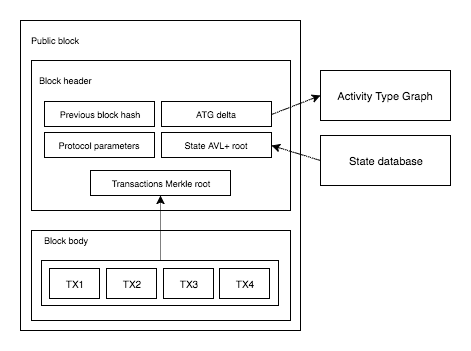
\includegraphics[width=0.8\textwidth]{public-blocks}
\caption{Public block structure}
\label{fig:publicblocks}
\end{figure}

There are two major ways to store the account balances and other state information: UTXO and account-based architectures. UTXO is an unspent transaction output, that contains some predicate -- a condition that has to be fulfilled in order to spend the coins. To prove the money ownership, the spender provides a witness -- an input that makes the predicate true. Thus, the UTXO-based architecture requires the transactions to be stateless, effectively limiting the application domain \cite{bentov2017instantaneous}.  The unspent outputs with an associated state can be treated as smart-contracts in the account-based architectures like Ethereum \cite{wood2014ethereum}. The state is stored in an off-chain storage -- the state database. The transactions are treated as the modifications of the world state.

Disciplina uses an account-based ledger with contracts programmable in Plutus language \cite{Plutus}. Each account has an associated state, which comprises the account balance and other information (e. g. log $L$ of a data disclosure contract). The world state is a mapping between accounts and their states. In order to make this mapping easily verifiable, we use a structure called the \textit{authenticated AVL+ tree} introduced in~\cite{reyzin2016improving}.

The recent achievements in the field of consensus protocols, like the provably secure Ouroboros \cite{kiayias2017ouroboros}, allow us to build a public chain based on the Proof of Stake consensus rules. Thus, we can increase the transaction speed and drop the need for the expensive mining.
